%!TEX root = ../username.tex
\chapter{Instance Segmentation And Evaluation Metrics} \label{chap:segmentation_metric}

The field of computer vision aims to enable machines the ability to comprehend and derive meaning from visual scenes. This field comprises several tasks for processing images and videos, including but not limited to image classification, object detection, semantic segmentation, and instance segmentation \cite{overview_cv_task}. However, for the purpose of our study, we will focus specifically on object detection and instance segmentation. In this section, we will define these two tasks, then compare them with related tasks such as image classification and semantic segmentation. Followed by a discussion of the metrics used to evaluate object detection and instance segmentation models.

\begin{figure}[!ht]
    \centering
    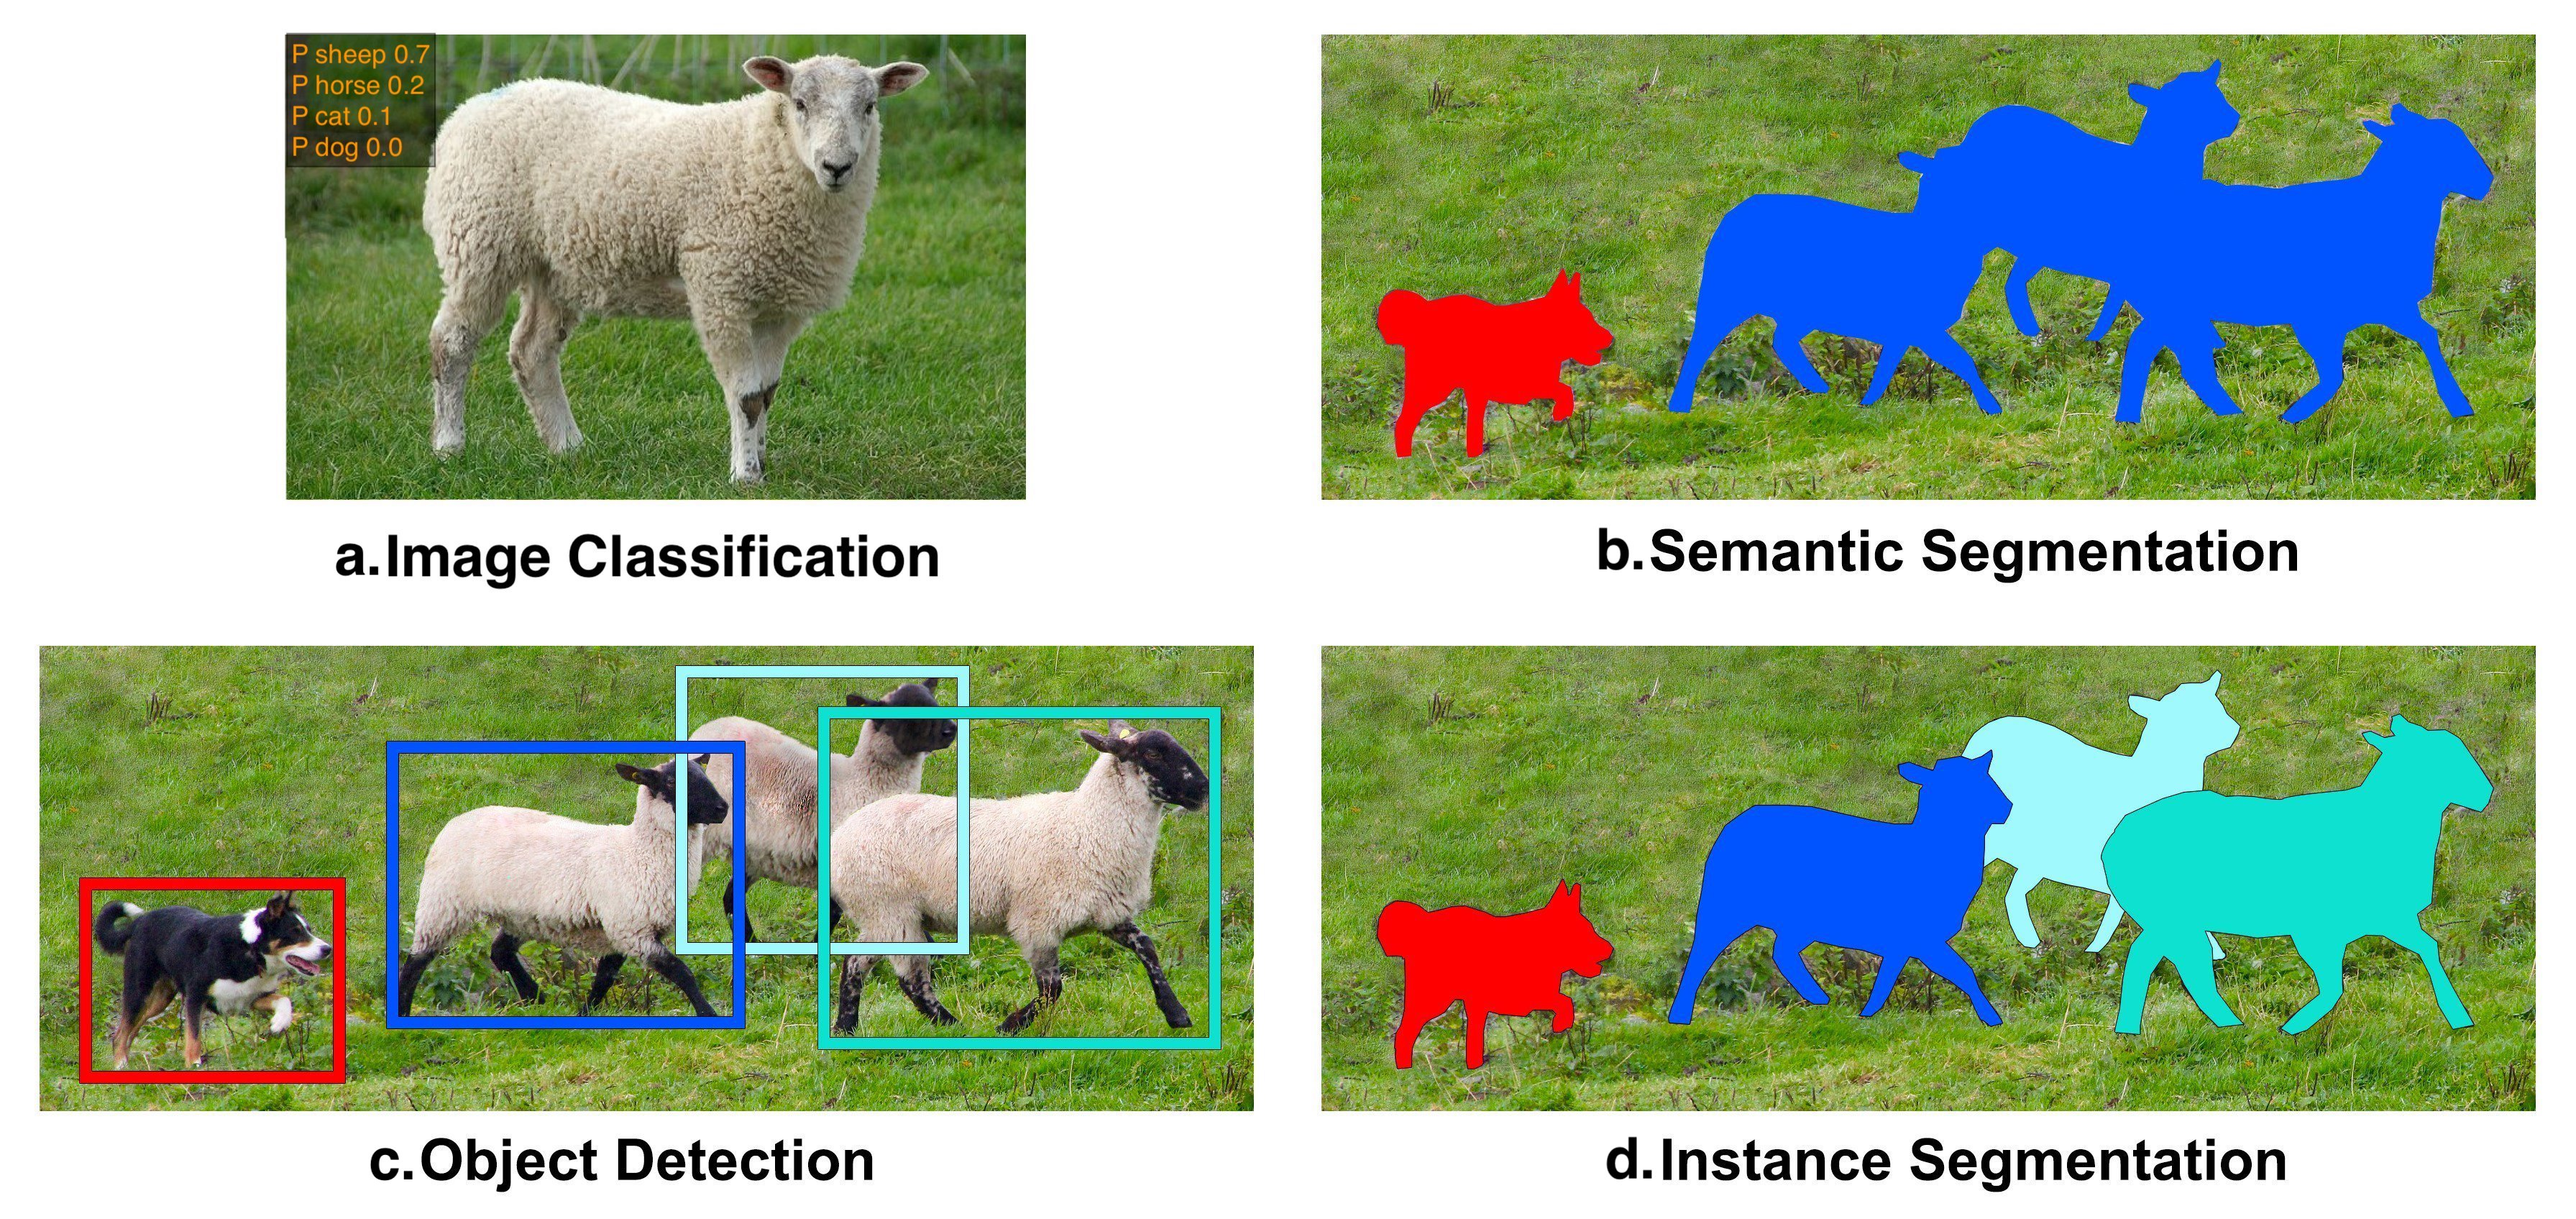
\includegraphics[width=4in]{figures/diff_cv_tasks.jpeg}
    \caption{Different Computer Vision Tasks \cite{diff_detection_segmentation_task_fig}}
    \label{fig:diff_cv_tasks}
\end{figure}

We begin with image classification, the most fundamental task in the computer vision field. The task involves assigning an object category label to an input image, assuming the input image contains exactly one object \cite{overview_cv_task}. This implies that the task allows the object classification label to be given to the entire image without specifying where the object is. As shown in Figure \ref{fig:diff_cv_tasks}a, the image classification model predicts the probability that the image shows a sheep, a horse, a cat, or a dog. Although image classification is comparatively simpler than other computer vision tasks, it presents several significant challenges due to the variability of image appearance caused by changes in scale, orientation, lighting, occlusions, and other factors.

The second task is semantic segmentation. In contrast to image classification, semantic segmentation is unconcerned with the presence or absence of objects in the input image. The objective of the task is to classify each pixel of the input image into one of several predefined classes or categories \cite{overview_cv_task}. By classifying each pixel, the task generates a detailed mapping between image pixels and classes that can be used to locate and outline objects of different classes within the image. However, when classifying each pixel without consideration of object location, the task removes the depth dimension of the image. That is, if two objects of the same class are positioned behind one another, then the semantic segmentation model will consider them as one object of this class, thus losing dimension information. Considering Figure \ref{fig:diff_cv_tasks}b, we noted the three sheep are at different locations in the depth dimension, but the semantic segmentation mask visualizes these sheep as one object in 2-dimensional space.

The third task is object detection, an improvement over image classification. The goal of object detection models is to locate and categorize each object within a given image \cite{overview_cv_task}. The process of object detection involves two main subtasks: object localization and object classification. Object localization determines the location and size of each object in an image by predicting a bounding box around the object. Once the object is localized, it can be classified using an image classification model. Compared to semantic segmentation, object detection retains all spatial information of the object in the image but loses the pixel accuracy mask. This is illustrated in Figures \ref{fig:diff_cv_tasks}c and \ref{fig:diff_cv_tasks}d, where object detection is able to detect all three sheep, but it is unclear whether a pixel within the bounding box refers to the sheep or the grass behind it.

The last task we want to discuss is instance segmentation. For every object in a given image or video frame, the instance segmentation model must identify all pixels belonging to the object and assign a category label to the object \cite{overview_cv_task}. Identifying all pixels that belong to the object creates the object's mask, which may then be used to locate pixel-precise locations and the object's outline. While object detection and instance segmentation involve locating objects, the former offers information about the location and scale of the detected objects, whereas the latter goes further by identifying all pixels associated with the object. On the other hand, the main distinction between instance and semantic segmentation lies in the level of detail they provide. While semantic segmentation divides an image into classes such as "vehicle" or "animal", instance segmentation provides more details by distinguishing between each individual object within those classes. It accomplishes this by assigning each object a unique label for identification. This means that instance segmentation can determine not only the class of each object in an image but also where it is located and how many there are - something semantic segmentation cannot achieve on its own. Considering Figure \ref{fig:diff_cv_tasks}, we observed that instance segmentation creates a pixel-accurate outline of all four animals, in contrast to the bounding box generated by object detection. In addition, the instance segmentation model's pixel-by-pixel mask must differentiate between the three sheep in contrast to semantic segmentation. In other words, the instance segmentation model combines object detection and semantic segmentation strengths while eliminating their weaknesses.


% Unlike semantic segmentation, which classifies each pixel in an image as belonging to a particular class, instance segmentation assigns a unique label to each object in a scene and then identifies its boundaries. For example, in a picture of two vehicles one after another on the street, instance segmentation distinguishes between the two vehicles by assigning them different labels and drawing a bounding box around them.

% The main distinction between instance and semantic segmentation lies in the level of detail they provide. While semantic segmentation divides an image into classes such as "vehicle" or "animal", instance segmentation provides more details by distinguishing between each individual object within those classes. It does this by assigning a unique label to each object for identification. This means that instance segmentation identifies not only what type of thing is present within an image but also where it is located and how many there are - something semantic segmentation cannot do on its own.

% However, instance segmentation and object detection are similar on a high level. Comparing instance segmentation with object detection tasks reveals further distinctions between the two tasks. While both involve locating objects within an image or video stream, object detection focuses on providing information about the location of the detected objects, while instance segmentation goes further by identifying their outlines as well as providing additional information about them, like the object size. Additionally, whereas object detection is used to detect multiple types of objects within one scene, instance segmentation is more focused on identifying individual instances within one specific type of object (e.g., two cars).

% According to the instance segmentation task definition, any model intending to complete this task must do two things. The model must first detect the object's location and draw a bounding box around it. Second, the model must determine the class of the object resigned within the bounding box defined in the previous step. In the second step, the model must also be aware of the number of instances for each class.

% In section \ref{sec:cnn}, we discussed the structure and building blocks of convolutional neural networks (CNNs). We also stated how CNNs classify objects in the image classification task in the discussion. However,  the image classification task assumes the image has exactly one object, and the model classifies the entire image based on that one object. Therefore, if we consider each bounding box as its own image, we can utilize a CNN to identify the object's class within the bounding box. This is the main idea behind the different variations of R-CNN, which is designed for object detection and instance segmentation task.  
R-CNN and YOLO are two popular families of models used for object detection and instance segmentation. In Sections 3 and 4, we will delve into the variations of R-CNN and YOLO, respectively. However, before we proceed, it is essential to understand the metrics used for assessing the performance of an object detection or instance segmentation model. In the next subsection, we will discuss the metrics utilized for evaluating these models.

\section{Evaluation Metrics}  \label{sec:eval_metrics}

As previously mentioned, an object detection model is responsible for localizing and classifying objects in an image by predicting a bounding box for each object and assigning a class label. Therefore, to evaluate the performance of an object detection model, the accuracy of the predicted bounding box and the given class label must be evaluated. Similarly, while evaluating an instance segmentation model, it is critical to analyze the quality of the pixel-wise mask in addition to the bounding box and category label. As a result, in this section, we will go over the metrics used to assess the accuracy of the bounding box, category label, and pixel-wise mask.

\subsection{Intersection over Union (IoU) Metric}  \label{subsec:iou_metric}
We start by discussing the evaluation metric for bounding box accuracy in the object detection task. In this task, the model predicts a bounding box for each object in the image to describe the object's location and size. The bounding boxes are commonly represented as a tuple $(x_{min},\ y_{min},\ x_{max},\ y_{max})$ indicating the coordinates of the top-left and bottom-right corners of the box. To evaluate the accuracy of the predicted bounding box, we compare its coordinates with the coordinate of a ground-truth bounding box. Each ground-truth bounding box is a manually annotated rectangle that precisely encloses an object in the image or video frame. With the ground-truth boxes, \textbf{Intersection over Union (IoU)}, also known as the Jaccard index or Jaccard similarity coefficient, the metric for measuring the degree of overlap between the predicted bounding box and the ground-truth bounding box for a given object \cite{generalized_iou}. In other words, given two rectangles represent the predicted bounding box and the ground-truth box, then the IoU can be expressed as:
\begin{equation}
    \text{IoU} = \frac{Area(BB_p \cap BB_t)}{Area(BB_p \cup BB_t)} \label{eq:iou}
\end{equation}
where $BB_p$ is the predicted bounding box, and $BB_t$ is the ground-truth bounding box. The IoU metric is defined in the range [0, 1], where a value closer to 0 indicates no overlap between bounding boxes, and 1 indicates a perfect overlap. Since $Area_{rectangle} = height \times width$, by comparing the area of two rectangles, the IoU metric incorporates the size and aspect ratio of the two boxes in comparison. As a result, the IoU metric is invariant to the size and aspect ratio. Due to its simplicity and invariance properties, IoU is widely used to measure the accuracy of predicted bounding boxes in various computer vision tasks \cite{generalized_iou}. Despite its success as a metric, IoU has a major weakness that prevents it from being used as a loss function. As shown in Equation \ref{eq:iou}, we noted that as long as the overlapping area is 0, i.e., $Area(BB_p \cap BB_t) = 0$, then IoU will be 0. In other words, when the predicted and ground-truth bounding boxes are not overlapping, the resulting IoU score does not indicate whether they are near or far from each other. The Generalized Intersection over Union (GIoU) was proposed to resolve this issue, as described in \cite{generalized_iou}.

\subsection{IoU Threshold and Confidence Threshold}  \label{subsec:iou_conf_threshold}
Next, we can assess the model's accuracy in classifying the object within each bounding box. Each bounding box requires the model to predict a categorical label and a confidence score. The label denotes the object's class within the bounding box, and the score reflects the model's confidence in identifying the object as belonging to this class. To assess the model's accuracy, we compare the predicted bounding box label with the ground-truth bounding box label. Before comparing the predicted box and ground-truth box labels, it is crucial to require that the degree of overlap between them meets a certain threshold $t_{IoU}$. If IoU $\geq t_{IoU}$, the detection is considered as a positive sample, whereas if IoU $< t_{IoU}$, the detection is considered as a negative sample. For each positive sample, we check if the model's confidence is higher than a predetermined threshold, $t_{confidence}$. If the confidence score meets the threshold, we compare the predicted label with the ground-truth label. Conversely, the comparison will result in a false if a bounding box is classified as a negative sample or has a confidence score lower than $t_{confidence}$. Therefore, to correctly classify a predicted bounding box, the model must satisfy three conditions: (1) the IoU score $\geq t_{IoU}$, (2) the confidence score $\geq t_{confidence}$, and (3) the predicted label matches the ground-truth label. If any of these conditions are not met, the model has incorrectly classified the predicted box.

The first condition (IoU score $\geq t_{IoU}$) is required because, assuming the second and third conditions are met, if the predicted bounding box and the ground-truth bounding box have little or no overlap, then the prediction should be considered false, and the model's accuracy should be reduced. The value of $t_{IoU}$ depends heavily on the task the model tries to accomplish. For tasks that require absolute precision, such as human surgery assistance, $t_{IoU}$ should be set high. However, a much lower threshold is more forgiving for tasks like checking the presence of a glass of water on the table. For evaluating the overall performance of the model, a $t_{IoU}$ value of 0.5 can be used, as demonstrated in the PASCAL VOC benchmark \cite{pascal_voc_2015}. Alternatively, the model can be evaluated at each $t_{IoU} \in \{0.50, 0.55, ..., 0.95\}$, as shown in the COCO benchmark \cite{coco_2014}. On the other hand, the second condition (confidence score $\geq t_{confidence}$) is necessary because the score directly affects the model's behavior in predicting accurately versus finding all occurrences. This behavior is denoted as the tradeoff between precision and recall, which we will discuss later in this section.

As an example, consider an image with 3 cars and 1 human. After processing the image with our object detection model, 2 cars and 1 human are identified with confidence scores of 0.76, 0.72, and 0.58, and IoU scores of 0.89, 0.32, and 0.52, respectively. The results are shown in the following table:
\begin{table}[H]
    \centering
    \begin{tabular}{rcccc}
        ground-truth labels         & car  & car  & car  & human \\ \hline
        predicted labels            & car  & car  & none & human \\ \hline
        predicted confidence scores & 0.76 & 0.72 & 0    & 0.58  \\ \hline
        predicted IoU scores        & 0.89 & 0.32 & 0    & 0.52 
    \end{tabular}
    \caption{Example's representation: Input image contains 3 cars and 1 human. The model predicts 2 cars and 1 human with respective confidence scores of 0.76, 0.72, and 0.58, and IoU scores of 0.89, 0.32, and 0.52} \label{ex:truth_pred_score_map}
\end{table}

Assuming the confidence threshold $t_{confidence}=0.6$, any predicted bounding box with confidence score lower than 0.2 will be removed. Additionally, assuming the IoU threshold $t_{IoU}=0.5$, then the truth bouding box with IoU score lower than 0.5 will be removed \cite{metrics_survey_2020}. In this example, one of the predicted car is 68\% offset from its truth location, hence the corresponding truth car label being removed. Thus the predicted labels and ground-truth labels are mapped one to one as follows:
\begin{table}[H]
    \centering
    \begin{tabular}{rcccc}
    ground-truth labels         & car  & none & car  & human \\ \hline
    predicted labels            & car  & car  & none & none
    \end{tabular}
\end{table}

\noindent Please note that changes in IoU and confidence thresholds can impact the correspondence between predicted and truth labels. For instance, if the IoU threshold ($t_{IoU}$) is adjusted to 0.7, the model will only recognize the first car as a ground-truth object, while the second car and human object (sample) will not be recognized. Similarly, if the confidence threshold ($t_{confidence}$) is set to 0.8, the model will not be able to detect any object, resulting in all predicted labels being classified as None. Therefore, it can be said that the value of $t_{IoU}$ determines whether a truth label is considered in the comparison, while $t_{confidence}$ determines whether a predicted label is considered in the comparison \cite{metrics_survey_2020}.

\subsection{Confusion Matrix}  \label{subsec:confusion_matrix}
The mapping between the predicted and ground-truth labels offers insight into the model's ability to detect and classify samples at a particular confidence and IoU threshold. We can quantify this insight using a confusion matrix, a 2 x 2 matrix that assesses the object detection model's performance in distinguishing between two categories \cite{confusion_matrix_2017}. Since the confusion matrix assumes that there are only two categories, when multiple categories are in the mapping, each category will have its unique confusion matrix. In other words, for each category, the confusion matrix measures the model's ability to differentiate between samples belonging to this category and those that do not. The confusion matrix comprises four different combinations of predicted and ground-truth labels, as shown:
\begin{table}[H]
    \centering
    \begin{tabular}{cc|cc|}
    \cline{3-4}
                                                        &          & \multicolumn{2}{c|}{Predicted}                                 \\ \cline{3-4} 
                                                        &          & \multicolumn{1}{c|}{Negative}            & Positive            \\ \hline
    \multicolumn{1}{|c|}{\multirow{2}{*}{Ground-Truth}} & Negative & \multicolumn{1}{c|}{True Negative (TN)}  & False Positive (FP) \\ \cline{2-4} 
    \multicolumn{1}{|c|}{}                              & Positive & \multicolumn{1}{c|}{False Negative (FN)} & True Positive (TP)  \\ \hline
    \end{tabular}
\end{table}

The \textbf{true negative (TN)} represents the count of times the model correctly recognizes a sample not belonging to a specific class. On the other hand, the \textbf{false negative (FN)} represents the number of ground-truth samples where the model fails to detect an object of this class at that position. The \textbf{false positive (FP)} is the count of samples that the model identifies as objects of this class at that position where there is no object or the IoU score is low. Lastly, the \textbf{true positive (TP)} denotes the number of ground-truth samples accurately recognized by the model. Consider Example \ref{ex:truth_pred_score_map}. Since we have two classes, we will have a confusion matrix for each class. Take the car class, for example, then:
\begin{itemize}
    \item True negative: The number of times the model \emph{correctly} classifies \emph{a none-car object as not a car}.
    \item False negative: The number of times the model \emph{incorrectly} classifies \emph{a car object as not a car}.
    \item False positive: The number of times the model \emph{incorrectly} classifies \emph{a none-car object as a car} or classifies \emph{a car object as a car but at a wrong location}.
    \item True positive: The number of times the model \emph{correctly} classifies \emph{a car object as a car}.
\end{itemize}
By utilizing these definitions, we can create the confusion matrix for the car class and, similarly, for the human class, with thresholds $t_{IoU}=0.5$ and $t_{confidence}=0.6$ as follow:
\begin{table}[H]
    \centering
    \begin{tabular}{cccc}
        \multicolumn{4}{c}{Confusion Matrix for Car Class} \\ \cline{3-4} 
                                                                                                          & \multicolumn{1}{c|}{}         & \multicolumn{2}{c|}{Predicted}                                \\ \cline{3-4} 
                                                                                                          & \multicolumn{1}{c|}{}         & \multicolumn{1}{c|}{Negative} & \multicolumn{1}{c|}{Positive} \\ \hline
        \multicolumn{1}{|c|}{\multirow{2}{*}{\begin{tabular}[c]{@{}c@{}}Ground\\ Truth\end{tabular}}}     & \multicolumn{1}{c|}{Negative} & \multicolumn{1}{c|}{1}        & \multicolumn{1}{c|}{1}        \\ \cline{2-4} 
        \multicolumn{1}{|c|}{}                                                                            & \multicolumn{1}{c|}{Positive} & \multicolumn{1}{c|}{1}        & \multicolumn{1}{c|}{1}        \\ \hline
    \end{tabular}
    \qquad
    \begin{tabular}{cccc}
        \multicolumn{4}{c}{Confusion Matrix for Human Class}                                                                                                                                              \\ \cline{3-4} 
                                                                                                          & \multicolumn{1}{c|}{}         & \multicolumn{2}{c|}{Predicted}                                \\ \cline{3-4} 
                                                                                                          & \multicolumn{1}{c|}{}         & \multicolumn{1}{c|}{Negative} & \multicolumn{1}{c|}{Positive} \\ \hline
        \multicolumn{1}{|c|}{\multirow{2}{*}{\begin{tabular}[c]{@{}c@{}}Ground\\ Truth\end{tabular}}}     & \multicolumn{1}{c|}{Negative} & \multicolumn{1}{c|}{3}        & \multicolumn{1}{c|}{0}        \\ \cline{2-4} 
        \multicolumn{1}{|c|}{}                                                                            & \multicolumn{1}{c|}{Positive} & \multicolumn{1}{c|}{1}        & \multicolumn{1}{c|}{0}        \\ \hline
    \end{tabular}
\end{table}
\noindent where in the car confusion matrix, FP$=1$ because ground-truth label is "none" while predicted label is "car", FN$=1$ because ground-truth label is "car" while predicted label is "none", and TN$=1$ because both ground-truth and predicted label ("human" and "none", respectively) are not "car".

\subsection{Accuracy Metric}  \label{subsec:accuracy_metric}
With the confusion matrix, we can assess the overall object detection model's performance at a particular threshold by computing the accuracy, precision, and recall metrics. First, the \textbf{accuracy (ACC) metric} describes how the model performs in detecting and classifying samples of all known classes. It is determined by dividing the number of correct detections by the total number of predictions made \cite{szeliski_cv_book}, as follows:
\begin{equation}
    ACC = \frac{TN+TP}{TN+FN+TP+FP} \label{eq:accuracy}
\end{equation}
However, the accuracy (ACC) metric is only meaningful when all classes are equally important and the input data has an approximately equal number of samples belonging to each class. The ACC metric can be misleading when some specific classes dominate the input data. For example, suppose a model processes an image of 495 cars and 5 humans. If the model classifies all 500 detections as cars, then the ACC be $\frac{0+495}{0+0+495+5}=0.99$. This result indicates that the model is 99\% correct in detecting the presence of cars and humans, even though it was unable to detect any humans.

\subsection{Precision Metric}  \label{subsec:precision_metric}
An alternative metric that can be utilized is precision. \textbf{Precision metric} assesses the dependability of the model in identifying a detection as positive for a specific class \cite{metrics_survey_2020}. Unlike ACC, precision assesses the model's reliability in classifying a particular class rather than across all classes. Thus, the precision performance of the model is different for each class at a given threshold. Precision is defined in the range of $[0,1]$  as:
\begin{equation}
    Precision = \frac{TP}{TP+FP} \label{eq:precision}
\end{equation}
A precision score of 0 signifies that all samples identified by the model as belonging to this particular class are incorrect, while a score of 1 indicates that all predictions for this class are accurate. However, precision does not reflect instances where the model fails to identify some samples of this class. Take the car class in Table \ref{ex:truth_pred_score_map} as an example. Let assume the model correctly classify the seconf car as a car at a higher IoU value of 0.8, then the ground-truth and predicted labels correspondence map is:
\begin{table}[H]
    \centering
    \begin{tabular}{rcccc}
    ground-truth labels         & car  & car & car  & human \\ \hline
    predicted labels            & car  & car & none & none
    \end{tabular}
\end{table}
\noindent Therefore, the precision score for this class is $\frac{2}{2+0}=1$, indicating that when the model predicts a sample as a car, the ground-truth label for that sample is indeed a car 100\% of the time. However, it is worth noting that the precision score does not factor in the car that the model missed in our example.

\subsection{Recall Metric}  \label{subsec:recall_metric}
As previously stated, precision only measures the correctness of detections but not the model's ability to detect all samples of a particular class. \textbf{Recall metric} are often utilized in conjunction with precision to overcome this limitation. The recall is mathematically defined in the range of $[0,1]$ as:
\begin{equation}
    Recall = \frac{TP}{TP+FN} \label{eq:recall}
\end{equation}
A value of 0 denotes that the model has missed identifying all ground-truth samples belonging to this class, while a value of 1 indicates that the model has detected all ground-truth samples of this class \cite{metrics_survey_2020}. However, similar to other metrics, recall is not flawless, as it does not account for instances where the model classifies all negative samples as belonging to this class. For instance, consider the car class in Table \ref{ex:truth_pred_score_map}. If our model predicts all ground-truth samples as belonging to the car class, the car class's recall is $\frac{3}{3+0}=1$, suggesting that the model can identify all ground-truth cars. However, as illustrated, the recall value fails to account for the model's misclassification of a non-car (human) object as a car. This error can be detected by the false positive (FP) term in the precision metric. Therefore, precision and recall are typically used together to evaluate an object detection model.

Using the definition of precision and recall, we noted that the two metrics measure the model's accuracy in classifying objects of a particular class at a particular confidence threshold $t_{confidence}$. We denote objects belonging to this class referred to as positive samples, while those that do not belong are negative samples. Based on Equation \ref{eq:precision}, we can see that as the precision approaches 1, the true positive (TP) term increase while the false positive (FP) term decrease. This implies that the model becomes more confident in classifying a sample as positive as precision increases. On the other hand, Equation \ref{eq:recall} shows that as the true positive (TP) term increases and the false negative (FN) term decreases, the recall approaches 1. This indicates that a higher recall value means the model identifies more samples as positive. 

\subsection{Precision-Recall Curve}  \label{subsec:pr_curve}
As it might be seen, there is a tradeoff between precision and recall. Suppose we establish a high $t_{confidence}$ value for the model and only classify a sample as positive when its confidence score surpasses this threshold. In this case, the model may miss multiple ground-truth positive samples, resulting in high precision but low recall. Conversely, suppose we set a low $t_{confidence}$ value; then, the model may classify most samples as positive, even those that are incorrectly classified, resulting in the model having low precision but high recall. Nonetheless, an object detector is deemed as high performance at a particular IoU threshold if its precision remains high as its recall increases \cite{metrics_survey_2020}. Since the model's precision and recall vary depending on the confidence threshold $t_{confidence}$, we can calculate both metrics for each threshold value to examine the tradeoff between optimizing for one over the other. These computed metric values can be plotted on a two-dimensional plane to visualize the tradeoff, also known as the \textbf{precision-recall curve}. Figure \ref{fig:precision-recall_curve} shows examples of the precision-recall curve for a dataset and how the curve change at different IoU threshold value.

\begin{figure}[!ht]
    \centering
    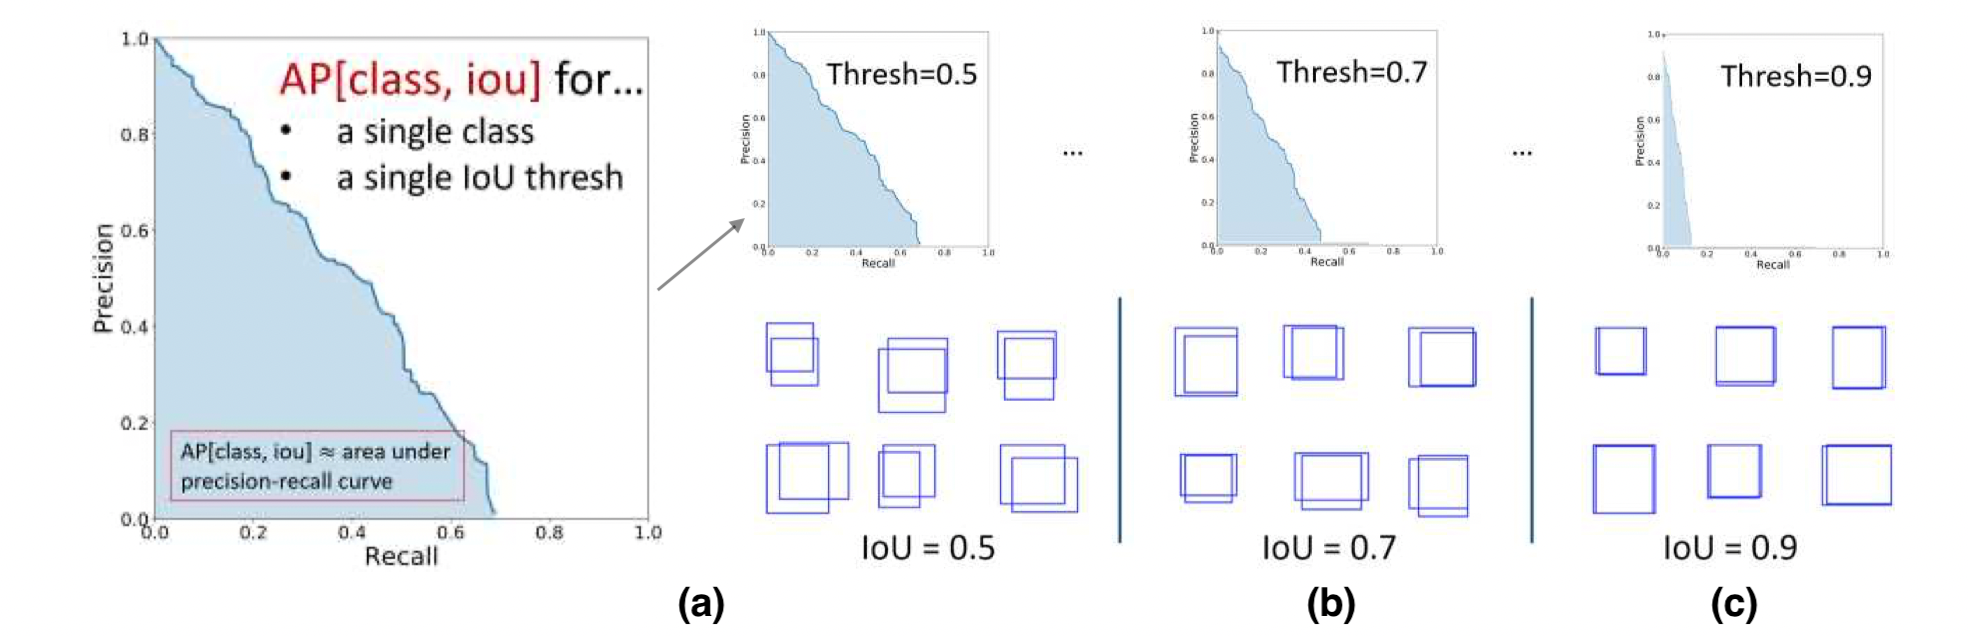
\includegraphics[width=5.5in]{figures/precision_recall_curve.png}
    \caption{\textbf{(a)} The precision-recall curve for a single class at the IoU threshold of 0.5 for a dataset. \textbf{(b, c)} the same precision-recall curve as (a) but with IoU threshold of 0.7 and 0.9, respectively. \cite{szeliski_cv_book}} 
    \label{fig:precision-recall_curve}
\end{figure}

\subsection{F-score (F1-score) Metric}  \label{subsec:f_score}
Optimizing a model for precision or recall, similar to choosing an IoU threshold value, heavily depends on the task the model tries to complete. If the model is used for a high-accuracy and detailed task, such as surgery, it should be optimized for precision metrics. On the other hand, if the task is more focused on catching as many instances as possible, such as low-cost home-based cancer diagnosis, the model should be optimized for recall. In cases where both precision and recall are equally important, we can determine the optimal combination of the two metrics by comparing their F-scores at different confidence thresholds. The F-score is the harmonic mean, a type of numerical average, of the precision and recall metrics \cite{fscore_2017}. For each pair of precision and recall, the F-score can be calculated as follows:
\begin{equation}
    \text{F-score} = 2 \times \frac{Precision \times Recall}{Precision + Recall}
\end{equation}
Given that the F-score is the harmonic mean of precision and recall metrics for a specific class at a confidence threshold $t_{confidence}$, comparing the F-score at different $t_{confidence}$ value help determine the optimal combination of precision and recall. The highest F-score obtained represents this optimal combination, allowing us to select the ideal confidence threshold value.

\subsection{Average Precision (AP) Metric}  \label{subsec:ap_metric}
Another metric that can be used to evaluate the performance of a model for each class is the average precision (AP). While the F-score describes the confidence threshold value at which the model achieves the highest performance for a particular class, the average precision (AP) summarizes the model's performance across various confidence thresholds for that class. In other words, the AP condenses the precision-recall curve for a specific class into a single value representing the average of all precisions. The AP is an estimate of the area under the precision-recall curve. There are different versions of AP; the adopted version for PASCAL VOC and COCO benchmark is the N-point interpolation AP \cite{n_point_interpolation_ap}. Let $P$ and $R$ denote precision and recall, respectively. The N-point interpolation AP is defined as follows:
\begin{equation}
    AP_N = \frac{1}{N} \sum_{R \in \mathbb{R}_N} P_{interp}(R) \qquad with \qquad P_{interp}(R) = \max_{{R}':{R}' \geq R} P({R}')
\end{equation}
where the set of $N$ interpolation $\mathbb{R}_N$ is $\left\{0, \frac{1}{N}, \frac{2}{N}, ..., \frac{N}{N}\right\}$. The term $P({R}')$ is the value of precision at recall ${R}'$. The condition $\max_{{R}':{R}' \geq R}$ implies that the $P_{interp}(R)$ is the highest precision value among all recall point ${R}'$ that are larger than $R$, instead of being the precision observed at the recall $R$ \cite{n_point_interpolation_ap}. As an example, consider using 11-point interpolation to the precision-recall curve shown in Figure \ref{fig:11AP_ex}. With this precision-recall curve, the 11-point interpolation AP is:
\begin{equation*}
    AP_{11} = \frac{1}{11} (1+0.666+3 \times 0.428 + 6 \times 0) \approx 26.818\% 
\end{equation*}
We noted that instead of using the precision value at each recall in $\left\{0, \frac{1}{10}, \frac{2}{10}, ..., \frac{10}{10}\right\}$, the $AP_{11}$ use the maximum precision value of all the remaining recall points. While the N-point interpolation technique simplifies the computation of the average precision (AP), it is an approximation method that yields a non-differentiable AP value. The difficulties in optimizing non-differentiable values make it challenging to use AP as a loss function. To address this limitation, recent research has proposed metrics like probability-based detection quality (PDQ) and Smooth-AP \cite{pdq_metric_2020, smoth_ap_metric_2020}.

\begin{figure}[!ht]
    \centering
    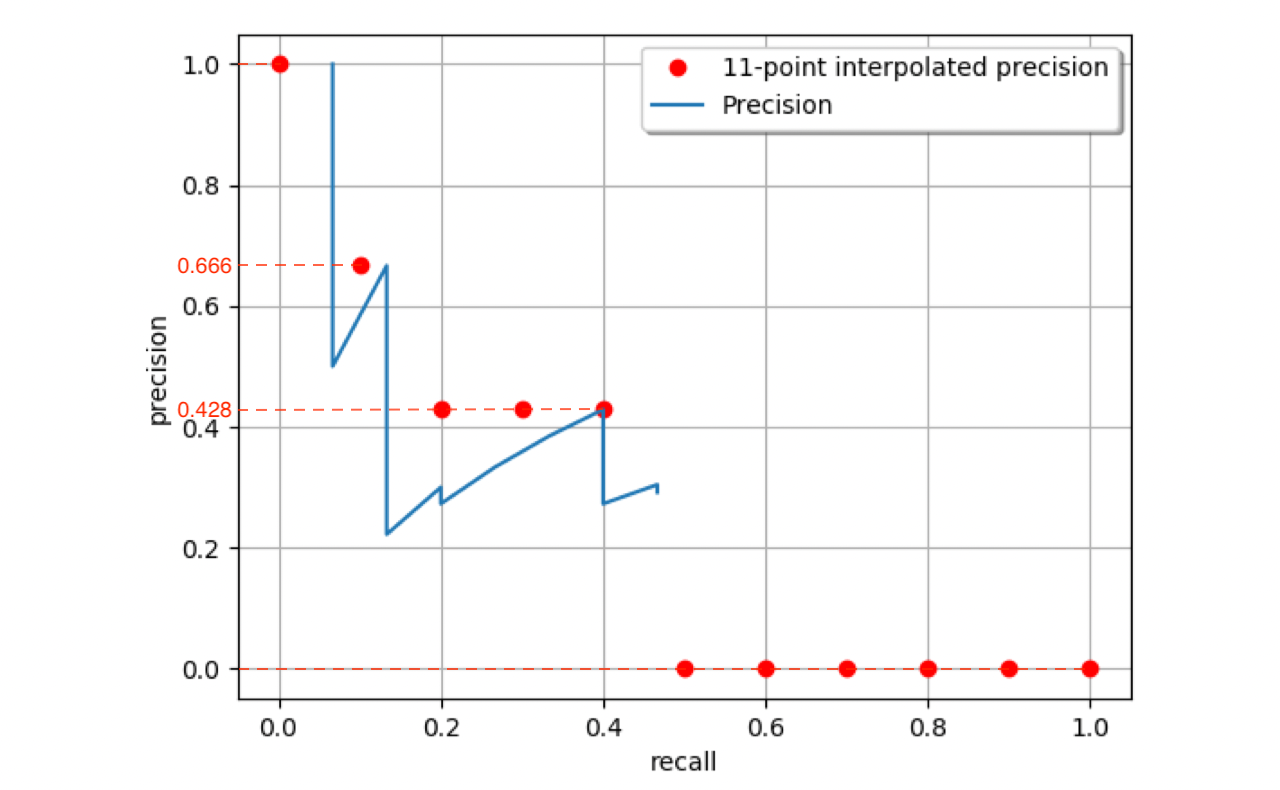
\includegraphics[width=4in]{figures/11AP_ex.png}
    \caption{Applied 11-point interpolation method on the precision-recall curve \cite{metrics_survey_2020}}
    \label{fig:11AP_ex}
\end{figure}

\subsection{Mean Average Precision (mAP) Metric}  \label{subsec:mean_ap_metric}
The mean average precision (mAP) of a class can be calculated using the average precision (AP) for that class at a specified IoU threshold \cite{szeliski_cv_book}. The mAP quantifies the model's accuracy in detecting objects of all classes above a particular IoU threshold. Let $K$ be the number of classes our model able to predict object for, then mAP is defined as follows:
\begin{equation}
    mAP = \frac{1}{K} \sum_{i=1}^{i=K}AP_i
\end{equation}
where $AP_i$ is the average precision value of the $i$th class.

In summary, evaluating object detection models is a five-step process. First, the Intersection over Union (IoU) between the predicted and ground-truth bounding boxes is calculated to determine the detection's location correctness. Second, a confusion matrix is created by comparing the predicted labels against the ground-truth labels at each IoU and confidence threshold. Third, the model's reliability and sensitivity can be quantified from the confusion matrix at each combination of the two thresholds by computing the precision and recall metrics. Moreover, the precision-recall curve and F-score can be computed to offer insights into the balance between the model's reliability and sensitivity. Fourth, the average precision (AP) metric is calculated to quantify the model's accuracy in detecting objects of a specific class at each IoU threshold. Finally, the mean average precision (mAP) metric represents the model's accuracy in detecting objects across all classes at a given IoU threshold. 

In comparison to object detection, instance segmentation models provide a more detailed output by generating a pixel-wise mask of the object, along with the object's bounding box and classification label. Therefore, to fully assess the performance of an instance segmentation model, we need to evaluate the accuracy of the detection at the pixel level. Similar to the bounding box, the accuracy of the object's mask can be measured using the Intersection over Union (IoU) metric, denoted as \emph{mask IoU} \cite{instance_segementation_metric_2022, mask_rcnn_2017}. The IoU for the object's mask is the ratio of overlapping pixels in the predicted and ground-truth masks over the total number of pixels in both. Consider representing the masks' bounding box as matrices, denoting a value of 1 to the pixels belonging to the object (i.e., inside the mask) and 0 to the pixels not (i.e., outside the mask). The union of the two mask matrices is the number of 1s in either matrix. The intersection is the number of 1s present in the output matrix of the element-wise product (Hadamard product) between the two masks' matrices. After computing the IoU for each pair of object masks, the subsequent steps for evaluating the model are identical to those used for object detection. This entails calculating the confusion matrix, precision-recall curve, F-score, AP, and mAP, but utilizing the mask's IoU rather than the bounding box's IoU.